\section{Improvement of the model}
\label{sec:improvement}
When we started to implement and simulate the model we found some fault
in the model, which gave rise to some ideas of how we make the model better.
These minor fault in the model and the solutions to have we could improve it
is described in this section.

\subsection{The repulsive force between agents in $ \Re ^{3}$}
From the given formula for calculating the repulsive force between agents in the 
description of the model, the part calculating the force to keep the personal space 
can be omitted when the agents are rather close to each other, then the calculation 
can be reduced as Equation (\ref{eq:re}).

\begin{equation}\label{eq:re}
\overrightarrow{f_{\alpha\beta}}(t) = A_{\alpha}^{2} exp\left[ \frac{r_{\alpha\beta} - d_{\alpha}\beta}{B_{\alpha}^{2}}\right]  \overrightarrow{n_{\alpha\beta}}
\end{equation}

Taking the norms of both sides of Equation (\ref{eq:re}), we can draw the relation 
between the value of $\overrightarrow{f_{\alpha\beta}}(t)$ and $d_{\alpha \beta}$, 
as in Figure (\ref{fig:physicalinteraction})
\\
\begin{figure}
\centering
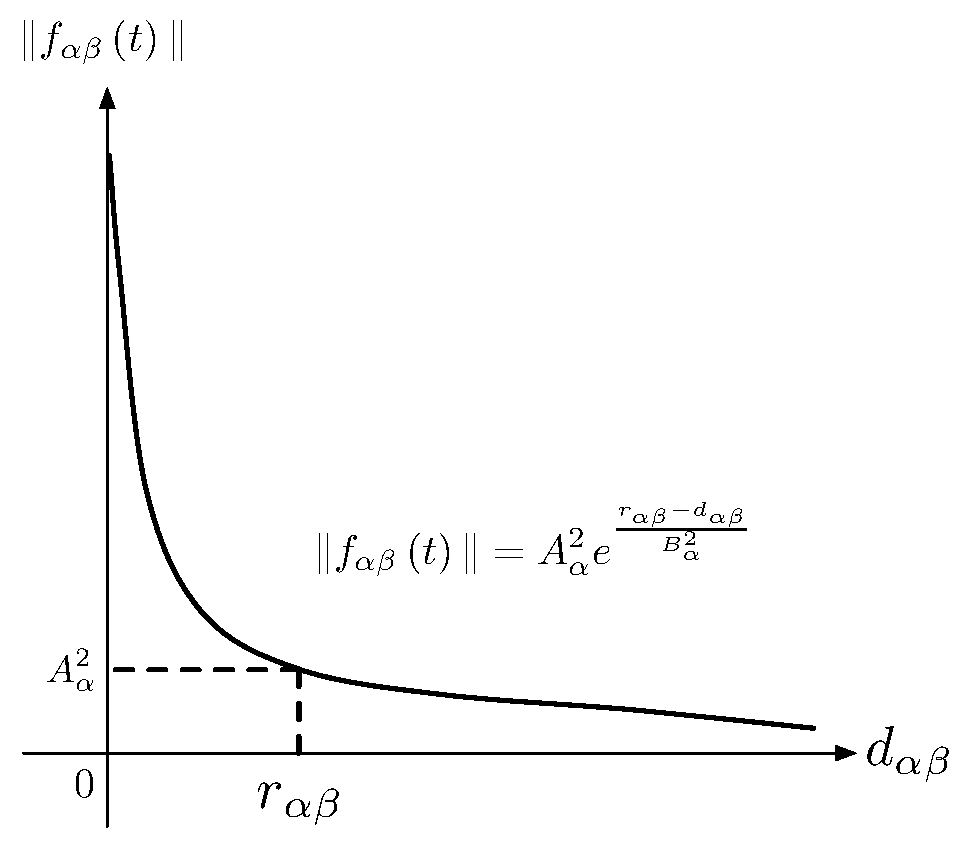
\includegraphics[scale=0.45]{Figures/physicalinteraction.pdf} 
\caption{The function about the interaction force $\vec{f_{\alpha\beta}}(t)$ and the distance between two agents
$d_{\alpha\beta}$ }\label{fig:physicalinteraction}
\end{figure}

There is one intersection of the graph and the axis $ \left( 0, A_{\alpha}^{2} exp\left( \frac{r_{\alpha\beta} }{B_{\alpha}^{2}}\right)  \right) $. 
If put into the constants, we will be able to get a maximum value of $ f_{\alpha\beta}(t) $, 
since the distance between agents cannot be negative. Here we set $ A_{\alpha}^{2} = 3 m/s^{2} $, 
$ r_{\alpha\beta} = 0.6 m $, and $ B_{\alpha}^{2} = 0.2 m $, so $ f_{\alpha\beta}(t)^{max} \doteq 60 m/s^{2} $, 
which is about six times the gravitational acceleration and represents a rather 
large force between agents (as large as six person's weight).

However, we notice that the effective part of the force calculated above is only the horizontal 
component that enables the agent to move horizontally in the plane where we do the simulation, 
but the reality is that the agents sometimes are also able to move vertically, for example, 
by stepping upon other people when they cannot take the pushing force from the surrounding agents. 
When that happens, the horizontal component of the repulsive force becomes smaller even if 
$d_{\alpha\beta}$ is kept the same.	
Therefore, a qualitative modification of dependence between $ f_{\alpha\beta}(t) $ 
and $ d_{\alpha\beta} $ could be:

\begin{figure}[hb]   
\centering
    {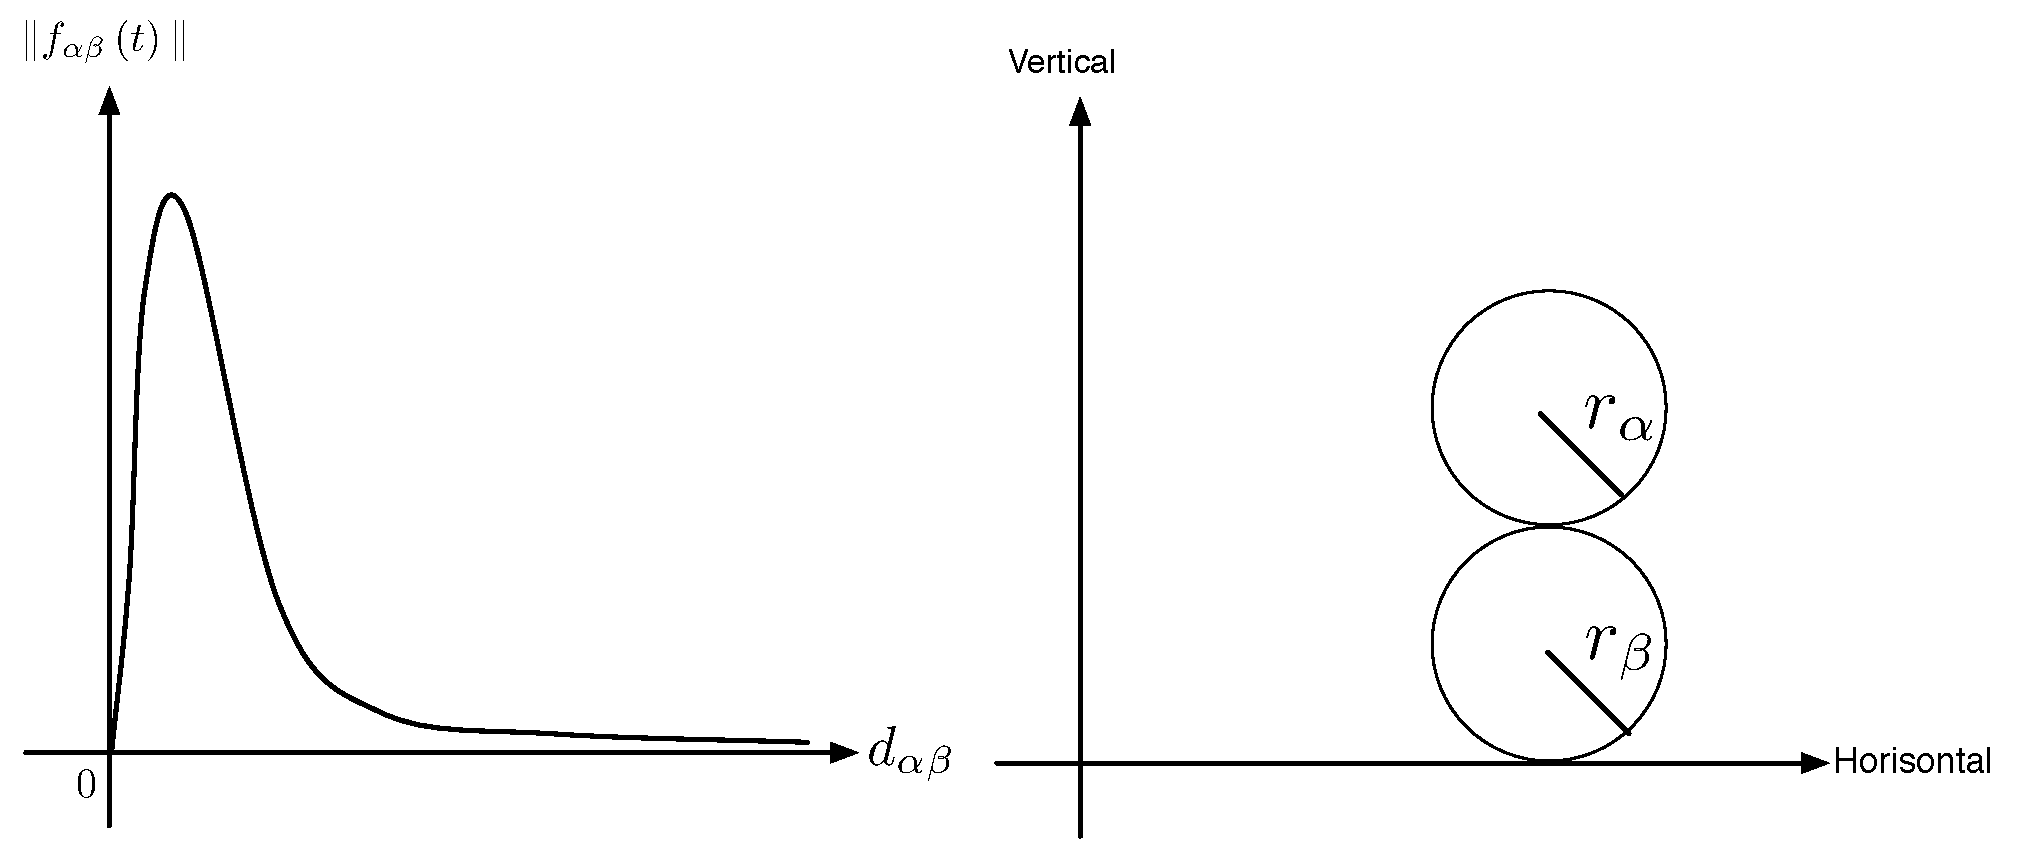
\includegraphics[scale=0.35]{Figures/ForceOverlapping.pdf}} 
    \caption{}
    \label{forceoverlapping}
\end{figure}
 
\subsection{Tangential forces}
Here we discuss the idea of improving the model by improving tangential forces, that is, the force parallel to the surface of an object.
The tangential forces can be used as collision avoidance, so that agents steer around obstacles or other agents \cite{tang}.
This would be relevant when simulating an environment where, e. g., and is standing in the middle of a symmetrical room and the agent's waypoint
is behind a big square pillar, with equal distance either way around, the agent would get stuck in front of the pillar without the tangential forces,
since the forces acting on the agent's motivation is cancelling each other out. 
In our case where two groups of agents are crossing each other in a corridor, the tangential force would make the agents to into account
the position of the agents in front of them and steer around them.

The tangential forces can also improve the model so it can simulate agents escaping a smoke filled room where we determine the visibility.
In this case of simulation the agents would walk randomly around untill they find a wall, and follow the wall around due to the tangential force.
This would be a way of implementing way finding to the model.

Friction between agents would also be possible to add to the model, since the tangential forces from other agents would make it
harder for agents to walk through a crowd. \cite{self-org} mention that friction is causing clogging in front of exits, since the people
get stuck in each other. In our simulation the agents are not clogging as heavily as \cite{self-org} mention it can be.
The time it take for the agent to leave a room in unrealistic low, and we think that implementing the friction by tangential forces
would make the simulation time more realistic.
